\pagebreak
\subsection{Cost and effort estimation: COCOMO II}

In this section we are going to estimate the effort (expressed in person-months), the number of people and the total time (expressed in months) required to complete the ``PowerEnJoy'' project.
We can do this using COCOMO II approach, which is a software cost estimation model used for estimating effort, cost and schedule of software projects. \\

COCOMO II is based on: 
\begin{itemize}
	\item \textbf{Source Line Of Code (SLOC)}
	\item \textbf{Scale Drivers (SD)}: their values determine the exponent used in the Effort Equation.
	\item \textbf{Cost Drivers (CD)}: their values determine the multiplicative factor used in the Effort Equation.
	\item \textbf{Effort Equation}: it estimates the effort measured in person-months
	\begin{center}
		 Effort = 2.94 * EAF * (KSLOC)$^{E}$
	\end{center}
	where: \\
	\textbf{EAF}: Effort Adjustment Factor derived from the Cost Drivers \\
	\textbf{E}: exponent derived from the values of the Scale Drivers
	
	\item \textbf{Schedule Equation}: it predicts the number of months that are required to complete the software project 
	\begin{center}
		Duration = 3.67 * (Effort)$^{SE}$ \\
	\end{center}
	where: \\
	\textbf{Effort}: the result of the Effort Equation \\
	\textbf{SE}: schedule equation exponent derived from the values of the Scale Drivers
\end{itemize}

%SCALE DRIVERS
\subsubsection{Scale Drivers}

Description of Scale Drivers:
\begin{itemize}
	\item \textbf{Precedentedness}: if a product is similar to several previously developed projects, then the precedentedness	is high. \\ Since we haven't any previous experience with this kind of projects, this value will be \textit{low}.
	\item \textbf{Development Flexibility}: if there are no specific constraints to conform to pre-established requirements and external interface specifications, then the development flexibility is high. \\ Since for this project there are requirements not too much detailed and no specification for the technology to be used, this value will be \textit{nominal}.
	\item \textbf{Architecture / Risk Resolution}: if we have a good risk management plan, clear definition of budget and schedule, focus on architectural definition, then the risk resolution is high. \\ Since the risk analysis we performed is quite extensive, then the value will be set to \textit{nominal}.
	\item \textbf{Team Cohesion}: if all stakeholders are able to work in a team and share the same vision and commitment, then the team cohesion is high. \\ Since in our team all the group members know each other and work together in a cooperative way, this value is \textit{high}.
	\item \textbf{Process Maturity}: refers to a well known method for assessing the maturity of a software organization. \\ We set this value to \textit{nominal}. 
\end{itemize}

In order to evaluate the values of the scale drivers, we refer to the following official COCOMO II table:
\begin{center}
	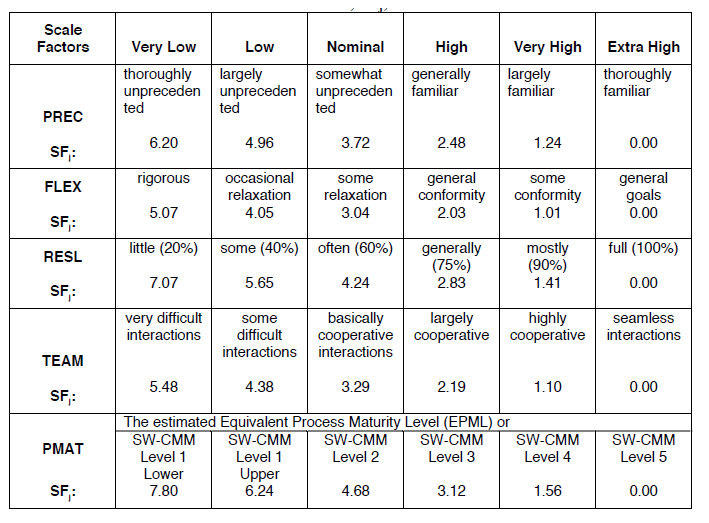
\includegraphics[width=\textwidth]{ScaleDriver}
\end{center}

The results of our evaluation are:
\begin{center}
	\begin{tabular}{l l c}
		\hline
		\textbf{Scale Driver} & \textbf{Factor} & \textbf{Value} \\
		\hline
		Precedentedness (PREC) & low & 4.96 \\
		Development Flexibility (FLEX) & nominal & 3.04 \\
		Risk Resolution (RESL) & nominal & 4.24 \\
		Team Cohesion (TEAM) & high & 2.19 \\
		Process Maturity (PMAT) & nominal & 2.68 \\
		\hline
		\textbf{Total} & & \textbf{17.11} \\
		\hline
	\end{tabular}
\end{center}

%COST DRIVERS
\subsubsection{Cost Drivers}

The selection of used cost drivers depend on whether we are in the case of post-architecture or early design. For \textbf{post-architecture} there are 16 different factors grouped in five categories: Product Factors, Platform factors, Personnel Factors, Project Factors and General Factor.\\
\\
\textbf{\underline{Product Factors:}}

\begin{itemize}
	\item \textbf{Required Software Reliability (RELY)}: this is the measure of the extent to which the software must perform its intended function over a period of time. If the effect of a software failure is only slight inconvenience then RELY is very low. If a failure would risk human life then RELY is very high. \\ Since ``PowerEnJoy'' isn't the only car sharing service in the city, a software failure could lead to important financial losses, then this value is set to \textit{high}.
\end{itemize}
	\begin{center}
		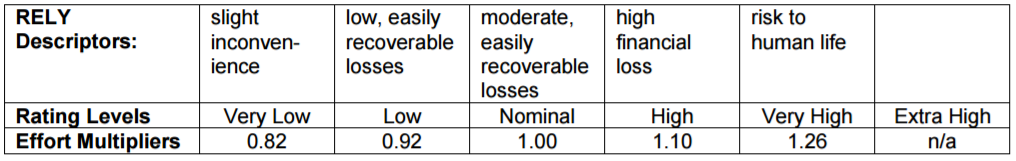
\includegraphics[width=\textwidth]{RELY}
	\end{center}

\begin{itemize}
	\item \textbf{Data Base Size (DATA)}: this measure consider the effective size of our database. this cost driver attempts to capture the effect large test data requirements have on product development. The rating is determined by calculating D/P, the ratio of bytes in the testing database to SLOC in the program. \\ We don't have the ultimate size of the database, but it might be about 1GB. Since the program size is equal to 12498 SLOC, the rate D/P is 80.012, then this value is set to \textit{nominal}. 
\end{itemize}
\begin{center}
	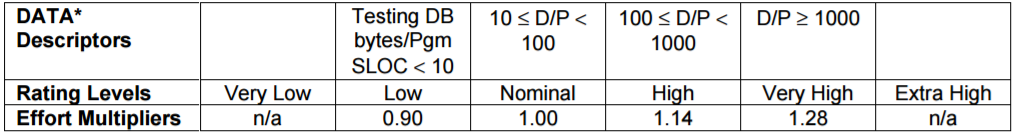
\includegraphics[width=\textwidth]{DATA}
\end{center}

\begin{itemize}
	\item \textbf{Product Complexity (CPLX)}: set to \textit{high} according to the new COCOMO II CPLEX rating scale.
\end{itemize}
\begin{center}
	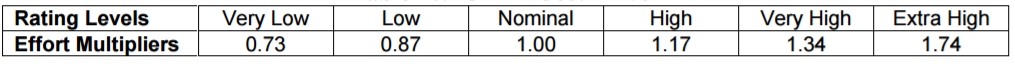
\includegraphics[width=\textwidth]{CPLX}
\end{center}	

\begin{itemize}
	\item \textbf{Developed for Reusability (RUSE)}: this cost driver accounts for the additional effort needed to construct components intended for reuse on current or future projects. This effort is consumed with creating more generic design of software, more elaborate documentation, and more extensive testing to ensure components are ready for use in other applications. \\ In our project there are some reusable components since we tried to design the system as modular as possible. Then the RUSE cost driver is \textit{nominal}.
\end{itemize}
\begin{center}
	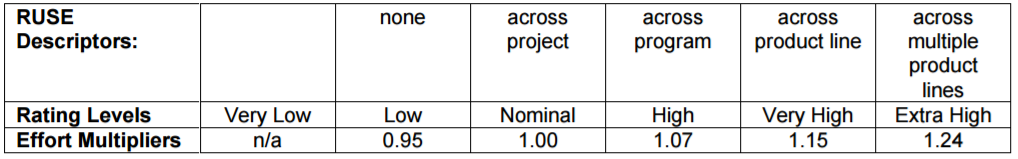
\includegraphics[width=\textwidth]{RUSE}
\end{center}

\begin{itemize}
	\item \textbf{Documentation Match to Life-Cycle Needs (DOCU)}: in COCOMO II, the rating scale for the DOCU cost driver is evaluated in terms of the suitability of the project’s documentation to its life-cycle needs. The rating scale goes from Very Low (many life-cycle needs uncovered) to Very High (very excessive for life-cycle needs). \\ In our case each aspect of the system os already described in the RASD, in the DD and in the ITPD, so the DOCU cost driver is set to \textit{nominal}.
\end{itemize}
\begin{center}
	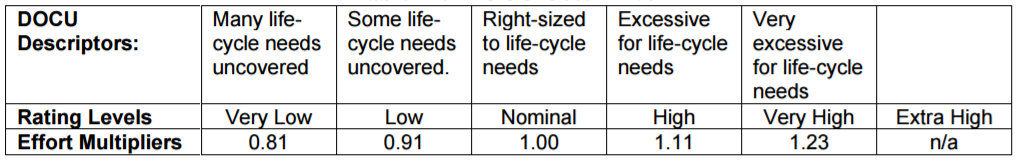
\includegraphics[width=\textwidth]{DOCU}
\end{center}
\textbf{\underline{Platform factors:}}

\begin{itemize}
	\item \textbf{Execution Time Constraint (TIME)}: this parameter describes the expected amount of CPU usage with respect to the computational capabilities of the hardware. The rating ranges from	nominal, less than 50\% of the execution time resource used, to extra high, 95\% of the execution time resource is consumed. \\Since our application is a complex piece of software, then the TIME value is \textit{high}.
\end{itemize}
\begin{center}
	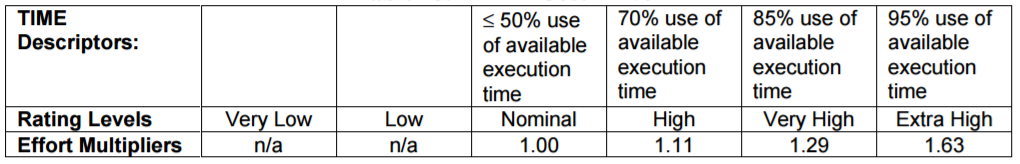
\includegraphics[width=\textwidth]{TIME}
\end{center}	

\begin{itemize}
	\item \textbf{Main Storage Constraint (STOR)}: this parameter describes the expected amount of storage usage with respect to the availability of the hardware. Since our storage availablity is of several terabytes, then the STOR value si \textit{nominal}.
\end{itemize}
\begin{center}
	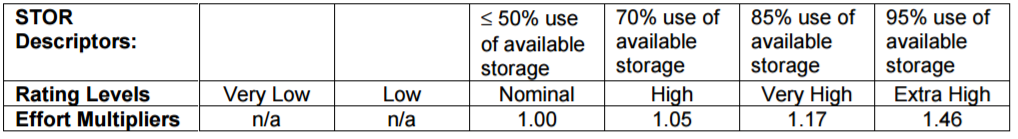
\includegraphics[width=\textwidth]{STOR}
\end{center}

\begin{itemize}
	\item \textbf{Platform Volatility (PVOL)}: ``Platform'' is used here to mean the complex of hardware and software (OS, DBMS, etc.) the software product calls on to perform its tasks. If the software to be developed is an operating system then the platform is the computer hardware. If a database management system is to be	developed then the platform is the hardware and the operating system. If a network text browser is to be developed then the platform is the network, computer hardware, the operating system, and the distributed information repositories. The platform includes any compilers or assemblers	supporting the development of the software system. This rating ranges from low, where there is	a major change every 12 months, to very high, where there is a major change every two weeks. \\ Since ``PowerEnJoy'' application shouldn't change too often: it could only require some updates once a year. Then the PVOL value is \textit{low}.
\end{itemize}
\begin{center}
	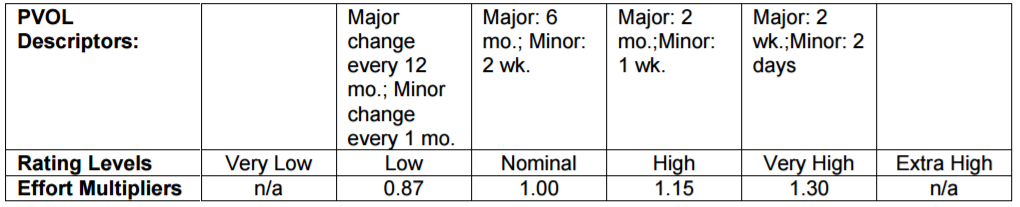
\includegraphics[width=\textwidth]{PVOL}
\end{center}
\textbf{\underline{Personnel Factors:}}

\begin{itemize}
	\item \textbf{Analyst Capability (ACAP)}: analysts are personnel who work on requirements, high-level design and detailed design.	The major attributes that should be considered in this rating are analysis and design ability,	efficiency and thoroughness, and the ability to communicate and cooperate. \\ Since we dedicated a lot of effort analysing the requirements problems keepeing in mind the possible real implementation. In particular, not only we can grant that the requirements have been correctly studied and accomplished, but also that our
	design makes our application actually useful for the user, providing all the basic functionalities he/she may need. In particular we resolved any ambiguity present in the initial description in the RASD. Then the ACAP value is set to \textit{high}.
\end{itemize}
\begin{center}
	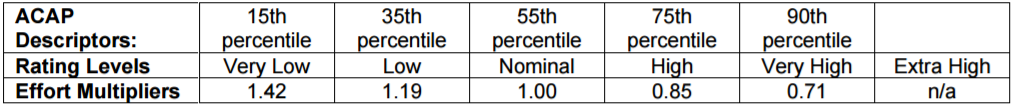
\includegraphics[width=\textwidth]{ACAP}
\end{center}	

\begin{itemize}
	\item \textbf{Programmer Capability (PCAP)}: evaluation should be based on the capability of the programmers as a team rather than as individuals. Major factors which should be considered in the rating are ability, efficiency and thoroughness, and the ability to communicate and cooperate. \\ We set the PCAP value to \textit{high}.
\end{itemize}
\begin{center}
	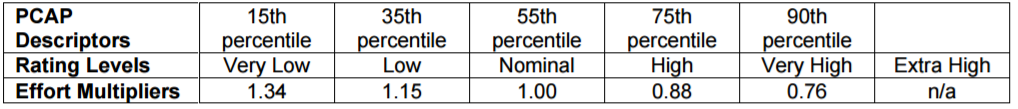
\includegraphics[width=\textwidth]{PCAP}
\end{center}	

\begin{itemize}
	\item \textbf{Personnel Continuity (PCON)}: the rating scale for PCON is in terms of the project’s annual personnel turnover: from 3\%, very high continuity, to 48\%, very low continuity. \\ Since the time we can spend on this project is limited and also the available time is less than a year, then this value is \textit{nominal}.
\end{itemize}
\begin{center}
	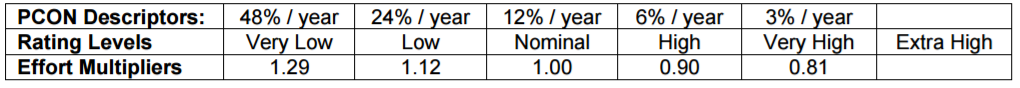
\includegraphics[width=\textwidth]{PCON}
\end{center}

\begin{itemize}
	\item \textbf{Applications Experience (APEX)}: the rating for this cost driver (formerly labeled AEXP) is dependent on the level of applications experience of the project team developing the software system or subsystem. The ratings are defined in terms of the project team's equivalent level of experience with this type of application. A very low rating is for application experience of less than 2 months. A very high rating is for experience of 6 years or more. \\ Since we haven't a lot of experience in this typology of project, then this value is equal to \textit{low}.
\end{itemize}
\begin{center}
	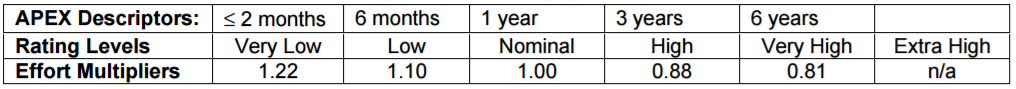
\includegraphics[width=\textwidth]{APEX}
\end{center}

\begin{itemize}
	\item \textbf{Platform Experience (PLEX)}: the Post-Architecture model broadens the productivity influence of platform experience, PLEX (formerly labeled PEXP), by recognizing the importance of understanding the use of more powerful platforms, including more graphic user interface, database, networking, and distributed middleware capabilities. \\ We have some experience with databases, user interfaces and server-side development, so this parameter value is \textit{nominal}. 
\end{itemize}
\begin{center}
	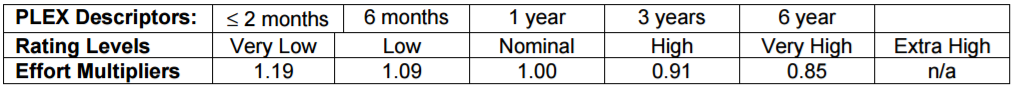
\includegraphics[width=\textwidth]{PLEX}
\end{center}

\begin{itemize}
	\item \textbf{Language and Tool Experience (LTEX)}: this is a measure of the level of programming language and software tool experience of the project team developing the software system or subsystem. Software development includes the use of tools that perform requirements and design representation and analysis, configuration management, document extraction, library management, program style and formatting,
	consistency checking, planning and control, etc. In addition to experience in the project’s	programming language, experience on the project’s supporting tool set also affects development effort. A low rating is given for experience of less than 2 months. A very high rating is given for experience of 6 or more years. \\ Since we have some experiences with JavaScript, databases, user interfaces and server-side development, then this value is \textit{nominal}.
\end{itemize}
\begin{center}
	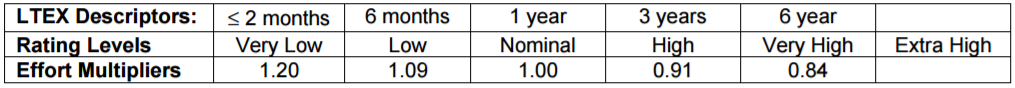
\includegraphics[width=\textwidth]{LTEX}
\end{center}
\textbf{\underline{Project Factors:}}

\begin{itemize}
	\item \textbf{Use of Software Tools (TOOL)}: the tool rating ranges from simple edit and code, very low, to integrated life-cycle management tools, very high. \\ Since our application environment is complete and well integrated, so this parameter value is \textit{high}.
\end{itemize}
\begin{center}
	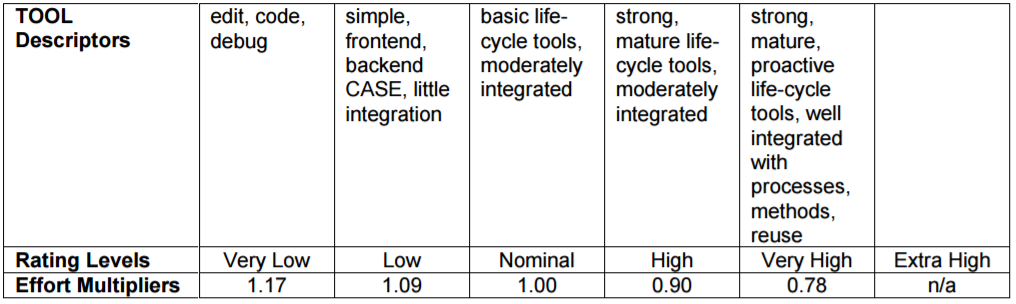
\includegraphics[width=\textwidth]{TOOL}
\end{center}

\begin{itemize}
	\item \textbf{Multisite Development (SITE)}: because of multisite development effects are significant, it's important to consider the SITE cost driver. Determining SITE cost driver rating involves the assessment and judgement-based averaging of two factors: site collocation (from fully collocated to international distribution) and communication	support (from surface mail and some phone access to full interactive multimedia). \\ We live in different cities, but we collaborate using phones, email and social networks. So we set this parameter to \textit{high}.
\end{itemize}
\begin{center}
	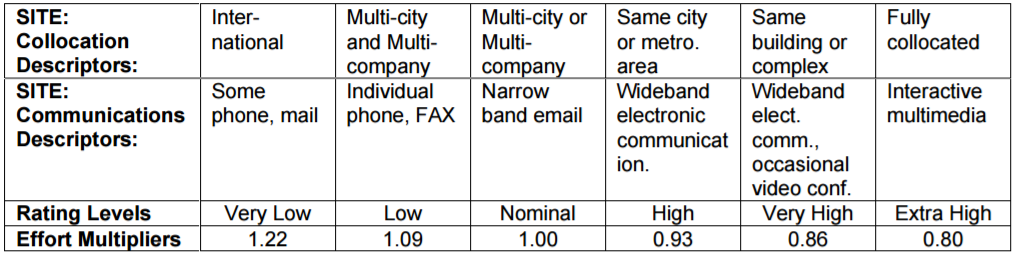
\includegraphics[width=\textwidth]{SITE}
\end{center}
\textbf{\underline{General Factors:}}

\begin{itemize}
	\item \textbf{Required Development Schedule (SCED)}: this rating measures the schedule constraint imposed on the project team developing the software. The ratings are defined in terms of the percentage of schedule stretch-out or acceleration with respect to a nominal schedule for a project requiring a given amount of effort. Accelerated schedules tend to produce more effort in the earlier phases to eliminate risks and refine the architecture, more effort in the later phases to accomplish more testing and
	documentation in parallel. \\ Our effort were well distribuited over the available time, but the requirements and design architecture analysis required a lot of time. Then this parameter value is \textit{high}.
\end{itemize}
\begin{center}
	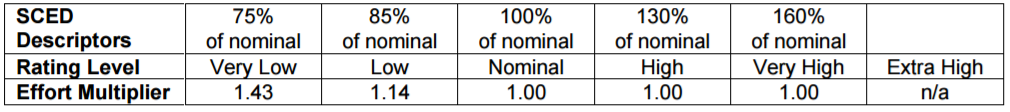
\includegraphics[width=\textwidth]{SCED}
\end{center}

\pagebreak
Here are our results:
\begin{center}
	\begin{tabular}{l l c}
		\hline
		\textbf{Cost Driver} & \textbf{Factor} & \textbf{Value} \\
		\hline \hline
		\underline{Product Factors} & & \\
		Required Software Reliability (RELY) & high & 1.10 \\
		Data Base Size (DATA) & nominal & 1.00 \\
		Product Complexity (CPLX) & high & 1.17 \\
		Developed for Reusability (RUSE) & nominal & 1.00 \\
		Documentation Match to Life-Cycle Needs (DOCU) & nominal & 1.00 \\
		\hline
		\underline{Platform Factors} & & \\
		Execution Time Constraint (TIME) & high & 1.11 \\
		Main Storage Constraint (STOR) & nominal & 1.00 \\
		Platform Volatility (PVOL) & low & 0.87 \\
		\hline
		\underline{Personnel Factors} & & \\
		Analyst Capability (ACAP) & high & 0.85 \\
		Programmer Capability (PCAP) & high & 0.88 \\
		Personnel Continuity (PCON) & nominal & 1.00 \\
		Applications Experience (APEX) & low & 1.10 \\
		Platform Experience (PLEX) & nominal & 1.00 \\
		Language and Tool Experience (LTEX) & nominal & 1.00 \\
		\hline
		\underline{Project Factors} & & \\
		Use of Software Tools (TOOL) & high & 0.90 \\
		Multisite Development (SITE) & high & 0.93 \\
		\hline
		\underline{General Factors} & & \\
		Required Development Schedule (SCED) & high & 1.00 \\
		\hline \hline
		\textbf{Total} & & \textbf{0.85593} \\
		\hline
	\end{tabular}
\end{center}

\pagebreak
%EFFORT EQUATION
\subsubsection{Effort Equation}

This equation gives us the effort estimation measured in Person-Months:
\begin{center}
	$ Effort := A * EAF * (KSLOC)^{E} $
\end{center}
where:
\begin{description}
	\item [A:] {2.94 (for COCOMO.2000) }
	\item [EAF:] {product of all the Cost Drivers, that in our case is: \textbf{0.85593}} 
	\item [E:] {exponent derived from Scale Drivers. It's calculated as:
		\begin{center}
			$ E := B + 0.01 * \sum_{j} SF_{j} $
		\end{center}
		that in our case is: 0.91 + 0.01 * \textbf{17.11} = \textbf{1.0811}\\ in which B is equal to 0.91 for COCOMO.2000.}
	\item [KLOC:] {estimated lines of code using the FP analysis, in our case are: \textbf{12.498}KLOC}
\end{description}
With thes parameters we can compute the \underline{Effort} value, that is equal to:
\begin{center}
	$ Effort = 2.94 * 0.85593 * 12.498^{1.0811} = \textbf{38.6 } PM \sim \textbf{39 } PM $
\end{center}

\vfill
%SCHEDULE ESTIMATION
\subsubsection{Schedule Estimation}

This equation gives us the schedule estimation measured in Month:
\begin{center}
	$ Duration := 3.67 * (Effort)^{SE}$ 
\end{center}
where: 
\begin{description}
	\item [Effort:] {the result of the Effort Equation, that in our case is \textbf{38.6}PM }
	\item [SE:] {schedule equation exponent derived from the values of the Scale Driver. It's calculated as:
		\begin{center}
			$ SE := 0.28 + 0.2 * (E - B) $
		\end{center}
	that in our case is: 0.28 + 0.2 * 0.1711 = \textbf{0.31422} }
\end{description}
With these parameters we can compute the \underline{Duration} value, that is equal to:
\begin{center}
	$ Duration = 3.67 * (38.6)^{0.31422} = \textbf{11.56 } months $ \\
\end{center}
